\documentclass[a4paper,12pt]{article}
\usepackage{hyperref}
\usepackage{graphicx}
\usepackage{subcaption}
\begin{document}
\title{\huge\bf Proyecto fase 1, Estad\'istica 2020-2021}
\author{Javier E. Dom\'inguez Hern\'andez C-312\\
        David Orlando de Quesada Oliva C-311\\
        Daniel de la Cruz Prieto C-311\\        
        }
\date{21 de marzo de 2021}
\maketitle


\textbf{\large\underline{Ejercicio 1}}\\

\noindent Para trabajar este ejercicio generamos una poblacion normal con media y desviaci\'on aleatorias
(La poblacion consiste en la estatura en metros de 500 personas).\\
\begin{enumerate}
    \item[a)] Muestra 1 de la poblac\'ion (mucho mayor que 30, con reemplazo): \\\\
1.91, 1.86, 2.22, 1.44,	1.47, 1.53,
1.35,	1.76,	1.62,	1.84,   1.76,	1.81,
1.76,	1.81,	1.69,	1.55,   1.68,	1.54,
1.45,	1.86,	1.66,	1.73,   1.45,	1.91,
1.54,	1.85,	1.72,	1.33,   1.46,	1.76,
2.1,    1.69,	1.22,	1.83,   1.61,	1.53,
1.47,	2.08,	1.77,	1.76,   2.08,	1.79,
1.48,	1.83,	1.86,	1.42,   1.59,	1.6,
1.71,	1.59,	1.32,	1.3	,   1.68,	1.58,
1.55,	1.7,    1.27,	1.66,   1.45,	1.33,
2.01,	1.75,	1.35,	1.62,   1.4,    2.2,
1.57,	1.96,	1.68,	1.86,   1.52,	1.58,
1.51,	2.22,	1.62,	1.48,   1.88,	1.99,
1.42,	1.87,	1.65,	2.12,   1.87,	1.55,
1.53,	1.36,	1.22,	1.66,   1.74,	1.52,
1.89,	1.62,	1.82,	1.54,   1.54,	1.68,
1.87,	1.67,	1.71,	1.57\\\\

\newpage
\textbf{\underline{Estad\'isticos}} \\

Medidas de tendencia central:\\\\
media = 1.6679\\
Interpretaci\'on: una persona promedio tiene una estatura 1.67m aproximadamente.\\
moda = 1.76\\
Interpretaci\'on: la mayor\'ia de las personas tiene una estatura de 1,76 aproximadamente\\
mediana = 1.66\\
Interpretación: La media de las personas tiene una estatura de 1.66 aproximadamente\\

Medidas de dispersi\'on:\\
desviaci\'on = 0.2225\\
varianza = 0.0495\\
coeficiente de variaci\'on = 0.1334\\

Medidas de posici\'on:\\
1er cuartil = 1.5275\\
2do cuartil = 1.66\\
3er cuartil = 1.8225\\

Intervalos de confianza:\\
intervalo de confianza de la media = [1.624291 ,  1.711509]\\
intervalo de confianza de la varianza = [0.038159 ,  0.0668]\\
Nivel de confianza asumido = 95$\%$, por lo que $\alpha$ = 0.05\\\\

Muestra 2 de la poblac\'ion (mayor que 30, con reemplazo): \\\\
1.72,	1.69,	1.69,	1.58,	1.69,	1.14,\\
1.29,	1.68,	1.97,	1.6	,   1.82,	1.61,\\
1.79,	1.76,	1.78,	2.33,	1.51,	1.3,\\
1.6,    1.14,	1.81,	1.54,	1.79,	1.18,\\
1.96,	1.66,	2.14,	1.77,	1.54,	1.87,\\
1.51,	1.65,	1.83,	1.79,	1.56,	1.68,\\
1.52,	1.81,	1.44,	1.71\\

\textbf{\underline{Estad\'isticos}} \\

Medidas de tendencia central:\\\\
media = 1.6613\\
Interpretaci\'on: una persona promedio tiene una estatura 1.66m aproximadamente.\\
moda = 1.69, 1.79\\
Interpretaci\'on: la mayor\'ia de las personas tiene una estatura de 1.69 o 1,79m aproximadamente\\
mediana = 1.685\\
Interpretación: La media de las personas tiene una estatura de 1.69m aproximadamente\\

Medidas de dispersi\'on:\\
desviaci\'on = 0.2434\\
varianza = 0.0593\\
coeficiente de variaci\'on = 0.1465\\

Medidas de posici\'on:\\
1er cuartil = 1.54\\
2do cuartil = 1.685\\
3er cuartil = 1.79\\

Intervalos de confianza:\\
intervalo de confianza de la media = [1.585871 ,  1.736729]\\
intervalo de confianza de la varianza = [0.039792 ,  0.097771]\\
Nivel de confianza asumido = 95$\%$, por lo que $\alpha$ = 0.05\\\\

\newpage
Muestra 3 de la poblac\'ion (20, con reemplazo): \\\\
1.69,	1.32,	1.42,	1.79,	1.6,    1.87,
1.76,	1.56,	1.18,	1.49,	1.18,	1.42,
2.06,	1.88,	1.84,	1.92,	2.08,	1.14,
1.89,	1.78\\

\textbf{\underline{Estad\'isticos}} \\

Medidas de tendencia central:\\\\
media =  1.6435\\
Interpretaci\'on: una persona promedio tiene una estatura 1.64m aproximadamente.\\
moda =  1.42, 1.18\\
Interpretaci\'on: la mayor\'ia de las personas tiene una estatura de 1.42m o 1.18 aproximadamente\\
mediana =  1.725\\
Interpretación: La media de las personas tiene una estatura de 1.73m aproximadamente\\

Medidas de dispersi\'on:\\
desviaci\'on = 0.2923\\
varianza =  0.0854\\
coeficiente de variaci\'on = 0.1779\\

Medidas de posici\'on:\\
1er cuartil = 1.42\\
2do cuartil = 1.725\\
3er cuartil = 1.8725\\

Intervalos de confianza:\\
intervalo de confianza de la media = [1.515396 ,  1.771604]\\
intervalo de confianza de la varianza = [0.049391 ,  0.182181]\\
Nivel de confianza asumido = 95$\%$, por lo que $\alpha$ = 0.05\\\\

Muestra 4 de la poblac\'ion (30, con reemplazo): \\\\

1.64,	1.84,	1.4,    1.3,    1.88,	1.76,
1.18,	1.59,	2.01,	1.57,	1.36,	1.47,
1.42,	1.49,	1.33,	1.66,	1.99,	1.41,
1.61,	1.82,	1.69,	1.61,	1.75,	1.74,
1.73,	1.46,	1.45,	1.35,	1.58,	1.87\\

\textbf{\underline{Estad\'isticos}} \\

Medidas de tendencia central:\\\\
media =  1.5987\\
Interpretaci\'on: una persona promedio tiene una estatura 1.6m aproximadamente.\\
moda =  1.61\\
Interpretaci\'on: la mayor\'ia de las personas tiene una estatura de 1.61m aproximadamente\\
mediana =  1.6\\
Interpretación: La media de las personas tiene una estatura de 1.60m aproximadamente\\

Medidas de dispersi\'on:\\
desviaci\'on = 0.213\\
varianza = 0.0454\\
coeficiente de variaci\'on = 0.1332\\

Medidas de posici\'on:\\
1er cuartil = 1.4275\\
2do cuartil = 1.6\\
3er cuartil = 1.7475\\

Intervalos de confianza:\\
intervalo de confianza de la media = [1.52248 ,  1.67492]\\
intervalo de confianza de la varianza = [0.028796 ,  0.082046]\\
Nivel de confianza asumido = 95$\%$, por lo que $\alpha$ = 0.05\\\\

Muestra 5 de la poblac\'ion (100, sin reemplazo): \\\\
1.29,	1.96,	1.56,	1.76,	1.5,    1.52,
1.87,	1.91,	1.48,	1.88,	2.18,	1.58,
1.44,	1.88,	1.69,	1.91,	1.6,    1.51,
1.68,	1.49,	1.67,	1.36,	1.69,	1.84,
1.73,	1.09,	1.79,	1.67,	1.47,	1.82,
1.53,	1.49,	1.75,	1.71,	1.13,	1.36,
1.79,	1.75,	1.61,	1.43,	1.58,	1.69,
1.91,	1.73,	1.66,	2,      1.72,	1.72,
1.53,	1.39,	1.45,	1.96,	1.88,	1.52,
1.59,	1.85,	1.46,	1.66,	1.89,	1.97,
1.87,	1.62,	1.48,	1.8,    1.87,	1.74,
1.5,    1.68,	1.32,	1.92,	1.65,	1.51,
1.59,	1.59,	1.6,    1.34,	1.68,	1.38,
1.91,	1.78,	1.64,	1.48,	2.33,	1.57,
1.79,	1.61,	1.78,	2.1,    1.61,	1.7,
1.71,	2.12,	1.3,    1.54,	1.67,	1.86,
1.9,    1.83,	2.13,	1.64

\textbf{\underline{Estad\'isticos}} \\

Medidas de tendencia central:\\\\
media = 1.6767\\
Interpretaci\'on: una persona promedio tiene una estatura 1.68m aproximadamente.\\
moda =  1.91\\
Interpretaci\'on: la mayor\'ia de las personas tiene una estatura de 1.91m aproximadamente\\
mediana =  1.6\\
Interpretación: La media de las personas tiene una estatura de 1.6m aproximadamente\\

Medidas de dispersi\'on:\\
desviaci\'on = 0.213\\
varianza = 0.0454\\
coeficiente de variaci\'on = 0.1332\\

Medidas de posici\'on:\\
1er cuartil = 1.4275\\
2do cuartil = 1.6\\
3er cuartil = 1.7475\\

Intervalos de confianza:\\
intervalo de confianza de la media = [1.52248 ,  1.67492]\\
intervalo de confianza de la varianza = [0.028796 ,  0.082046]\\
Nivel de confianza asumido = 95$\%$, por lo que $\alpha$ = 0.05\\\\
\item [c)] 
\begin{figure}[t!]
    \centering
    \begin{subfigure}[b]{0.4\linewidth}             
        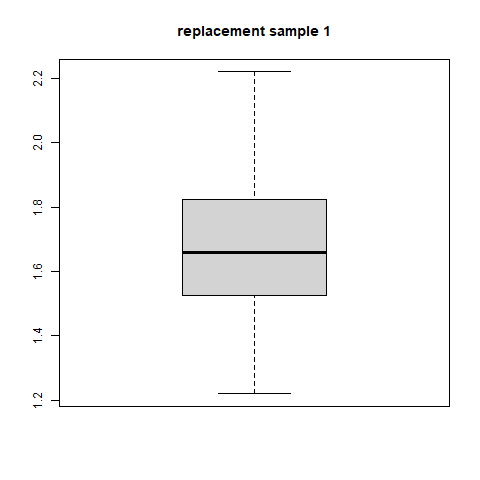
\includegraphics[width = \linewidth]{./datos generados (Ejercicio 1)/replacement_sample1_boxplot.png}
        \caption{cajas y bigotes}
    \end{subfigure}
    \begin{subfigure}[b]{0.4\linewidth}               
        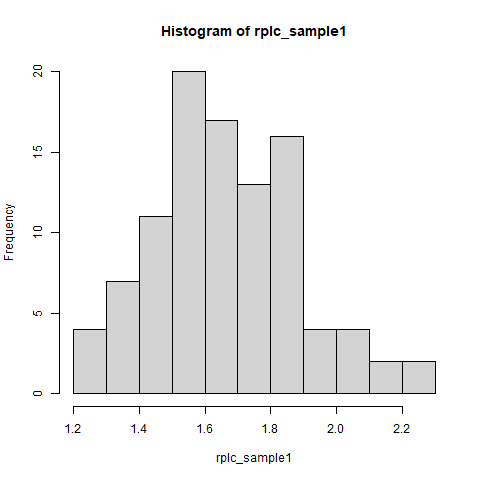
\includegraphics[width = \linewidth]{./datos generados (Ejercicio 1)/replacement_sample1_hist.png}
        \caption{histograma}
    \end{subfigure}

    
    \caption{Muestra1(con reemplazo)}
    \label{figure}
\end{figure}

\begin{figure}[t!]
    \centering
    \begin{subfigure}[b]{0.4\linewidth}             
        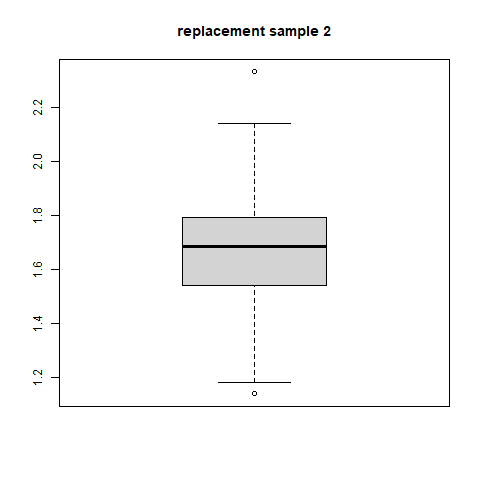
\includegraphics[width = \linewidth]{./datos generados (Ejercicio 1)/replacement_sample2_boxplot.png}
        \caption{cajas y bigotes}
    \end{subfigure}
    \begin{subfigure}[b]{0.4\linewidth}               
        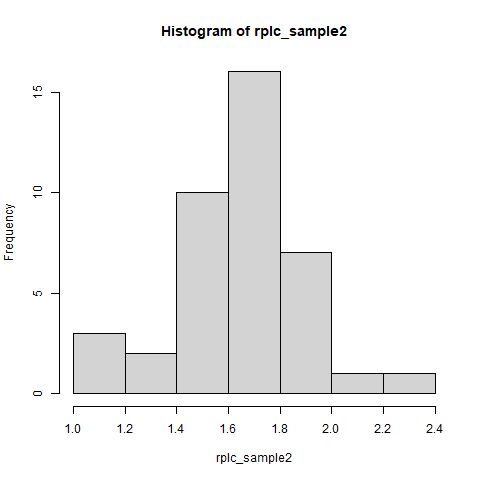
\includegraphics[width = \linewidth]{./datos generados (Ejercicio 1)/replacement_sample2_hist.png}
        \caption{histograma}
    \end{subfigure}

    
    \caption{Muestra2(con reemplazo)}
    \label{figure}
\end{figure}

\begin{figure}[t!]
    \centering
    \begin{subfigure}[b]{0.4\linewidth}             
        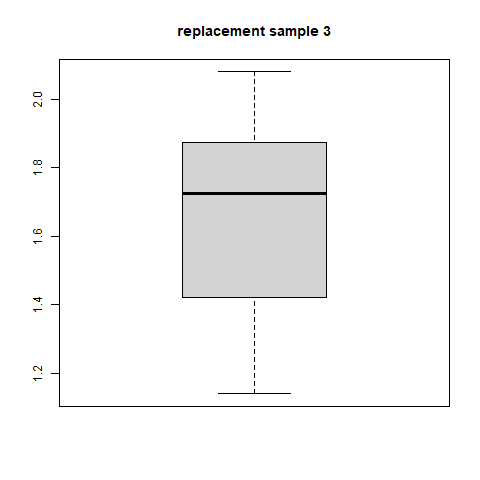
\includegraphics[width = \linewidth]{./datos generados (Ejercicio 1)/replacement_sample3_boxplot.png}
        \caption{cajas y bigotes}
    \end{subfigure}
    \begin{subfigure}[b]{0.4\linewidth}               
        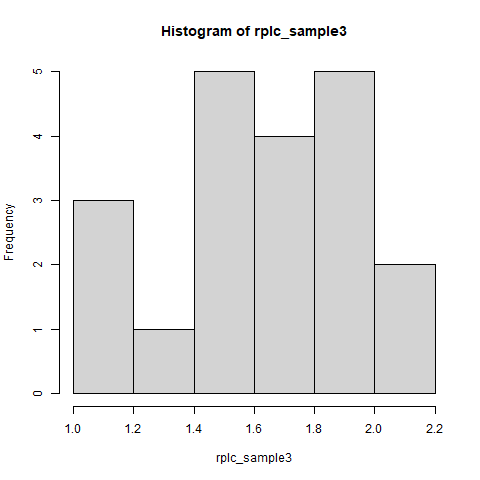
\includegraphics[width = \linewidth]{./datos generados (Ejercicio 1)/replacement_sample3_hist.png}
        \caption{histograma}
    \end{subfigure}

    
    \caption{Muestra3(con reemplazo)}
    \label{figure}
\end{figure}

\begin{figure}[t!]
    \centering
    \begin{subfigure}[b]{0.4\linewidth}             
        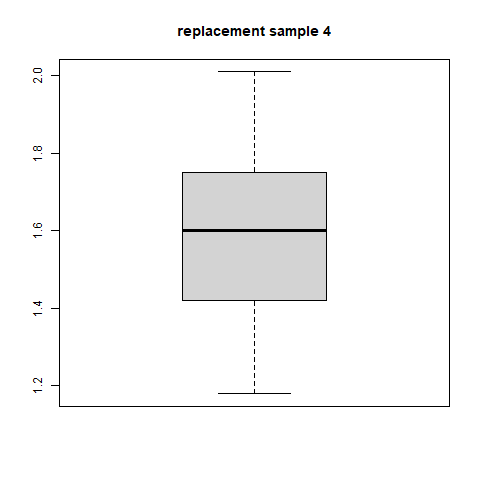
\includegraphics[width = \linewidth]{./datos generados (Ejercicio 1)/replacement_sample4_boxplot.png}
        \caption{cajas y bigotes}
    \end{subfigure}
    \begin{subfigure}[b]{0.4\linewidth}               
        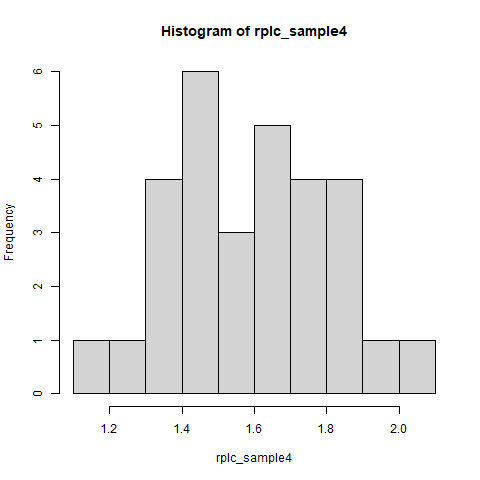
\includegraphics[width = \linewidth]{./datos generados (Ejercicio 1)/replacement_sample4_hist.png}
        \caption{histograma}
    \end{subfigure}

    
    \caption{Muestra4(con reemplazo)}
    \label{figure}
\end{figure}


\begin{figure}[t!]
    \centering
    \begin{subfigure}[b]{0.4\linewidth}             
        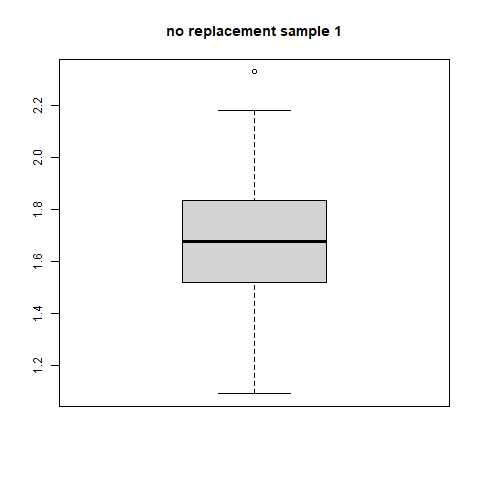
\includegraphics[width = \linewidth]{./datos generados (Ejercicio 1)/no_replacement_sample1_boxplot.png}
        \caption{cajas y bigotes}
    \end{subfigure}
    \begin{subfigure}[b]{0.4\linewidth}               
        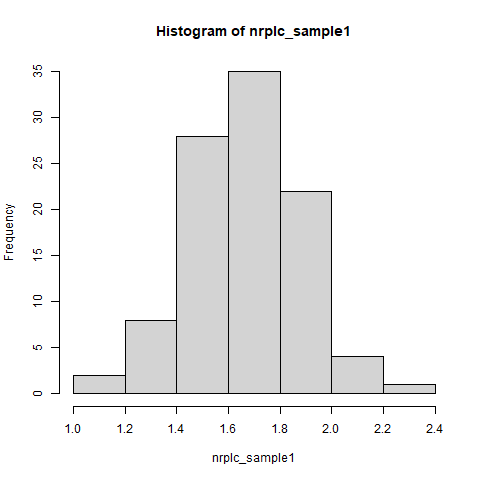
\includegraphics[width = \linewidth]{./datos generados (Ejercicio 1)/no_replacement_sample1_hist.png}
        \caption{histograma}
    \end{subfigure}

    
    \caption{Muestra5(sin reemplazo)}
    \label{figure}
\end{figure}

\begin{figure}[t!]
    \centering
    \begin{subfigure}[b]{0.4\linewidth}             
        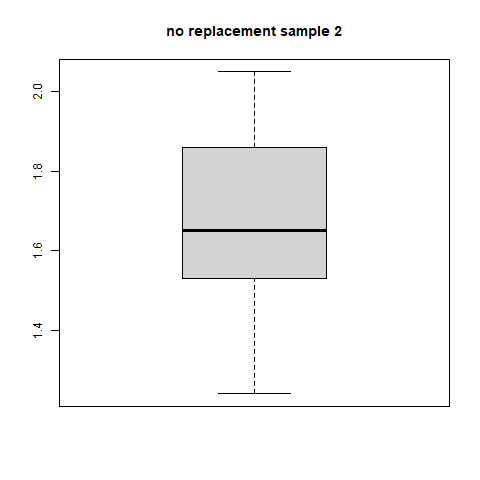
\includegraphics[width = \linewidth]{./datos generados (Ejercicio 1)/no_replacement_sample2_boxplot.png}
        \caption{cajas y bigotes}
    \end{subfigure}
    \begin{subfigure}[b]{0.4\linewidth}               
        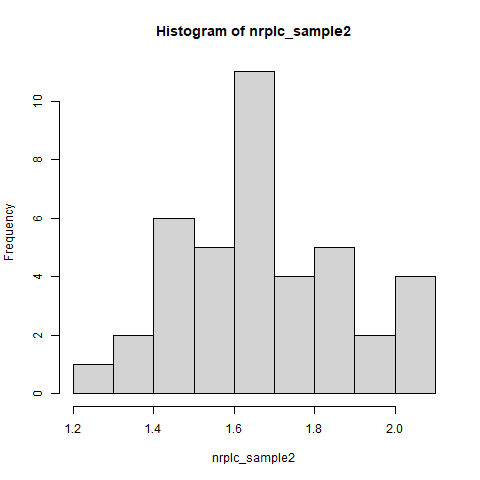
\includegraphics[width = \linewidth]{./datos generados (Ejercicio 1)/no_replacement_sample2_hist.png}
        \caption{histograma}
    \end{subfigure}

    
    \caption{Muestra6(sin reemplazo)}
    \label{figure}
\end{figure}

\begin{figure}[t!]
    \centering
    \begin{subfigure}[b]{0.4\linewidth}             
        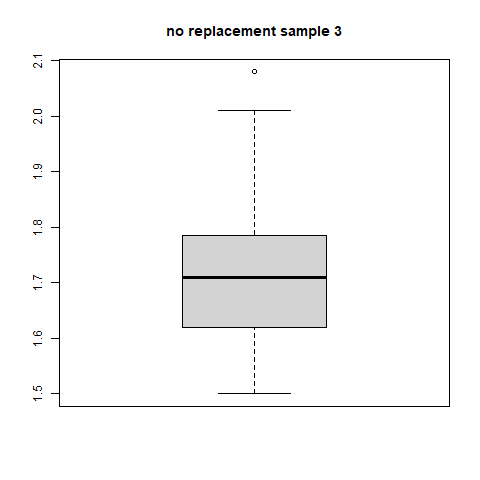
\includegraphics[width = \linewidth]{./datos generados (Ejercicio 1)/no_replacement_sample3_boxplot.png}
        \caption{cajas y bigotes}
    \end{subfigure}
    \begin{subfigure}[b]{0.4\linewidth}               
        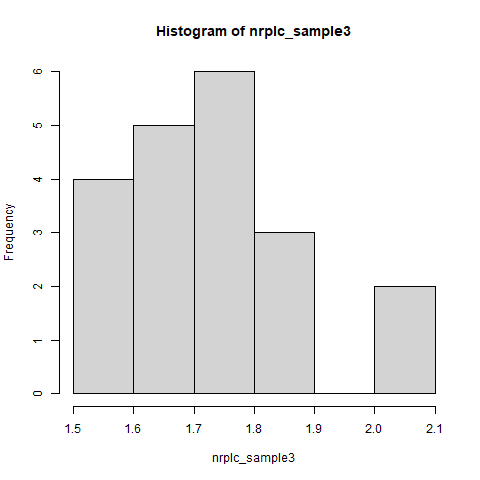
\includegraphics[width = \linewidth]{./datos generados (Ejercicio 1)/no_replacement_sample3_hist.png}
        \caption{histograma}
    \end{subfigure}

    
    \caption{Muestra7(sin reemplazo)}
    \label{figure}
\end{figure}

\begin{figure}[t!]
    \centering
    \begin{subfigure}[b]{0.4\linewidth}             
        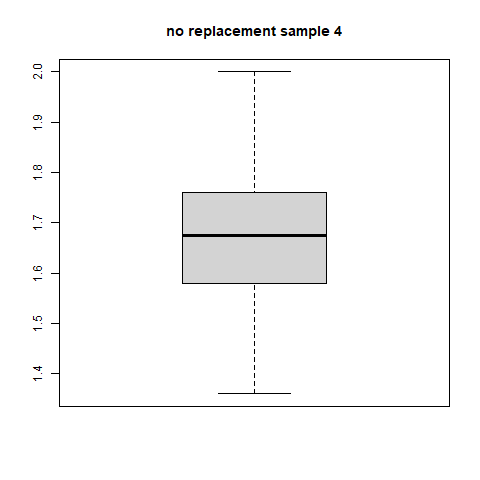
\includegraphics[width = \linewidth]{./datos generados (Ejercicio 1)/no_replacement_sample4_boxplot.png}
        \caption{cajas y bigotes}
    \end{subfigure}
    \begin{subfigure}[b]{0.4\linewidth}               
        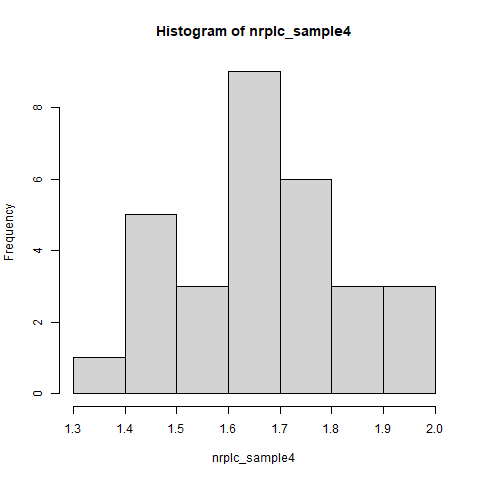
\includegraphics[width = \linewidth]{./datos generados (Ejercicio 1)/no_replacement_sample4_hist.png}
        \caption{histograma}
    \end{subfigure}

    
    \caption{Muestra8(sin reemplazo)}
    \label{figure}
\end{figure}


\end{enumerate}

%\begin{center}
%   \begin{tabular}{| c | c | c |}
%    \hline
%               & proa & centro & popa \\
%    producto A & 604 & 941 & 456 \\ \hline
%    producto B & 950 & 1278 & 772 \\ \hline
%    producto C & 446 & 781 & 272 \\ \hline
%    \hline
%    \end{tabular}
%\end{center}
\end{document}